\chapter{Dirichlet过程}
如今,使用概率模型来建模观察数据的分布已经成为了机器学习领域的主流方法。然而,当数据量和模型复杂度(通常指参数个数)不一致时,传统的参数模型会导致过拟合或者欠拟合的问题。常用的模型复杂度选择方法一般都需要人工进行,比如做多组实验进行交叉验证(cross validation)。非参数模型则通过在一个无限维的参数空间里寻找合适模型,使得参数的个数可以根据数据自动的调整来解决这一问题。近几年Guassian过程、Dirichlet过程等方法逐渐进入研究者的视野,许多相关的模型和算法被提出,并在某些应用上取得了良好的效果。本章主要介绍其中与Dirichlet过程相关的模型和算法。
\section{Dirichlet过程}
随机过程是定义在函数空间上的分布,它的每个采样都是一个概率测度。Dirichlet过程则是一种特殊的随机过程:如果对服从于某个随机过程的概率分布$G$,$G$在任何划分下都是服从Dirichlet分布的,则称该随机过程为Dirichlet过程。其严格定义如下: 

假设$G_0$是测度空间$\Theta$上的随机概率分布, $\alpha_0$是正实数, 对于测度空间$\Theta$上的概率分布$G$,如果其满足以下条件:

对测度空间$\Theta$的任意一个有限可测划分$(A_1,...,A_r)$,均有以下关系存在:
\begin{equation}
(G(A_1),...,G(A_r)) \sim Dir(\alpha_0G_0(A_1),..., \alpha_0G_0(A_r)) \label{eq:def_dp}
\end{equation}

则称$G$服从由基分布$G_0$和参数$\alpha_0$组成的Dirichlet过程(Dirichlet process,DP),记作$G  \sim DP(\alpha_0,G_0) $。根据Dirichlet分布的性质和式\eqref{eq:def_dp}可知,对于任意的$T \subset \Theta$,有:
\begin{equation}
\mathbb{E}[G(T)] = G_0(T) \label{eq:dp_mean_stat}
\end{equation}

所以$G_0$表征了其中心,而$a_0$表征了其分散程度.

反之, 如果满足$G  \sim DP(\alpha_0,G_0) $, 则有式\eqref{eq:def_dp}成立.

\subparagraph{共轭性}

与Dirichlet分布类似,Dirichlet过程具有共轭性,对于$G  \sim DP(\alpha_0,G_0) $,若观测到样本 $\theta \sim G$,根据Dirichlet分布的共轭性,有:
\begin{equation}
(G(A_1),...,G(A_r)|\theta \in A_k,\alpha_0,G_0) \sim Dir(\alpha_0G_0(A_1),..., \alpha_0G_0(A_k)+1,...,\alpha_0G_0(A_r)) 
\end{equation}
从而可知
\begin{equation}
p(G|\theta_1,...,\theta_N,\alpha_0,G_0) \sim DP(\alpha_0+N,\frac{1}{\alpha_0+N}(\alpha_0G_0+\sum_{i=1}^N\delta_{\theta_i})) \label{eq:dp_post}
\end{equation}

下面通过引入stick-breaking构造和中国餐馆过程,给出DP另外两个重要性质。

\subsection{Stick-breaking构造}

Ferguson证明了服从DP的测度是以概率1离散的\cite{Fer:73},Sethuraman给出了一种称为stick-breaking的方法,可以构造出服从DP的概率测度,直观的展示了这一性质。

按如下分布,生成两个独立的变量序列${\bm \beta}$和${\bm \theta}$:
\begin{equation}
\beta_k \sim Beta(1,\alpha_0), \theta_k \sim G_0 \quad k \in 1,...,\infty
\end{equation}

根据这两个变量序列,定义随机分布G:
\begin{equation}
\pi_k = \beta_k\prod_{l=1}^{k-1}(1 - \beta_l), G = \sum_{k=1}^{\infty}\pi_k\delta_{\theta_k}
\end{equation}
其中$Beta(1,\alpha_0)$是beta分布,$\delta_{\theta}$表示一个集中在点$\theta$处的概率测度(即在$\theta$处测度为1其他点测度均为0的一个概率测度)。Sethuraman证明了通过这一过程构造出的概率测度G服从$DP(\alpha_0,G_0)$。

这里需要注意,按照这一过程构造的序列$\pi$以概率1满足$\sum_{k=1}^{\infty}\pi_k = 1$。在文献中,通常用$\pi \sim GEM(\alpha_0)$表示$\pi$的构造。

\subsection{中国餐馆过程}
\subparagraph{预测分布}
对于一个服从DP分布的概率测度G,当已经观察到G的一系列采样$\phi_1,...\phi_N$时,考察对下个采样$\phi_{N+1}$的预测分布:
\begin{equation}
p(\phi_{N+1}|\phi_1,...,\phi_N,\alpha_0,G_0) = \int{p(\phi_{N+1}|G)p(G|\phi_1,...,\phi_N,\alpha_0,G_0)}dG
\end{equation}
上式右侧其实是$\mathbb{E}[G|\phi_1,...,\phi_n]$,根据式\eqref{eq:dp_mean_stat}和式\eqref{eq:dp_post},有:
\begin{equation}
p(\phi_{N+1}|\phi_1,...,\phi_N,\alpha_0,G_0) = \frac{1}{\alpha_0+N}(\sum_{i=1}^N\delta_{\phi_i} +\alpha_0G_0)\label{eq:polya_urn}
\end{equation}

这一预测分布对应的过程称为Blackwell-MacQueen Urn模型或者Polya Urn模型:假设有一个罐子,其中装有各种颜色的球(颜色可以重复),每次或者按等概率取出一个球,然后放回两个这一颜色的球,或者按照正比于$\alpha$的概率往罐子内放入一个新球(颜色可能是新的,也可能是罐子内已有)。
\begin{figure}
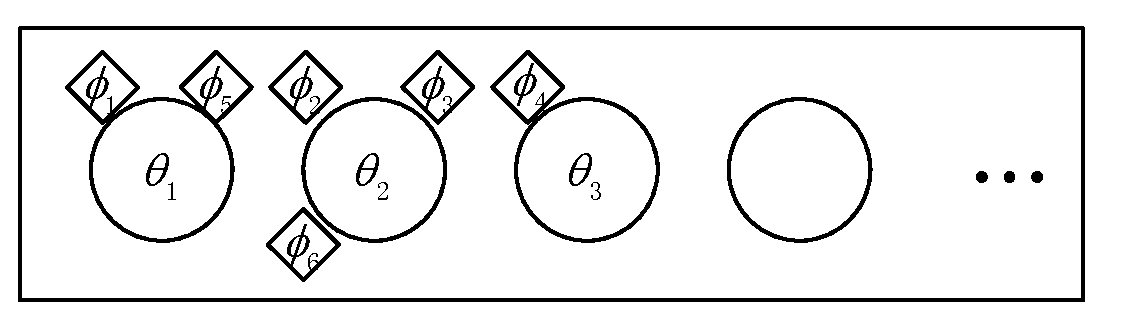
\includegraphics[angle=270,width=\textwidth]{CRP.pdf} 

  \caption{中国餐馆过程示意图} \label{fig:CRP}
\end{figure}
\subparagraph{中国餐馆过程}
上述的Polya urn模型中,$\phi$可能是重复的,故可以用$\theta_1$到$\theta_K$来表示$\phi_1$到$\phi_N$的所有可能的不同取值,进而重写式\eqref{eq:polya_urn}:
\begin{equation}
p(\phi_{N+1}|\phi_1,...,\phi_N,\alpha_0,G_0) = \frac{1}{\alpha_0+N}(\sum_{k=1}^KN_k\delta_{\theta_k} +\alpha_0G_0 ) \label{eq:crp_phi}
\end{equation}
其中$N_k$表示$\phi_i = \theta_k$的个数。
这个式子可以看出DP的聚类性质,即对于未观察的$\phi_{N+1}$,其和某些已有的$\phi_i$取相同值的概率是严格大于0的。
为了更好地表达此性质,这里定义一个用于指示类目的变量${\bm z}$,令$z_i = k$表示$\phi_i = \theta_k$,则有:
\begin{equation}
p(z_{N+1} = z |z_1,...,z_N,\alpha_0,G_0) = \frac{1}{\alpha_0+N}(\sum_{k=1}^KN_k\delta_k +\alpha_0\delta_{k^{new}}))\label{eq:crp_z}
\end{equation}
其中,$k^{new}$表示一个新的类。
Pitman和Dubins受到旧金山唐人街里几乎可以坐下无限人的中式餐馆的启发,将上述这个过程比喻为中国餐馆过程(Chinese restaurant process,CRP):假设有一家可以容纳无限张桌子的中国餐馆,每张桌子记为$\theta_k$,每位顾客记为$\phi_i$,第1个顾客就坐于第1张桌子,第$i$个顾客或者按正比于$n_k$(已经就坐于第k张桌子上的顾客数)的概率就坐于第$k$张桌子,或者按正比于$\alpha_0$的概率就坐于一张新桌子。图\ref{fig:CRP}直观的展示了这一过程。

可以看出,DP不仅具有聚类性质,而且他的聚类数是可以随着观察的增加而变化的,这正是其解决模型选择的关键所在。
\subparagraph{Antoniak定理}
Antoniak\cite{antoniak:74}证明了,如果知道当前的总样本数n(顾客数),其当前的不同成分个数m(桌子数)满足如下分布:
\begin{equation}
p(m|n,\alpha_0) \propto s(n,m)(\alpha_0)^m\frac{\Gamma(\alpha_0)}{\Gamma(\alpha_0+n)}  \label{eq:antoniak}
\end{equation}
其中s(n,m)为第一类Stirling数。表\ref{table:stirling_num}给出了Stirling数的一些值。其中$s(0,0)=1,s(n,0)=0,s(n,n)=1$,当$m>n$时,$s(n,m)=0$。其他情况下,$s(n+1,m)=s(n,m-1) + ns(n,m)$。

\begin{table}
\begin{center}\small
\begin{tabular}{l|lllll}
s(n,m) &m=0 & m=1 &  m=2 &  m=3 &  m=4 \\ \hline
n = 0 & 1 & 0 & 0 & 0 & 0 \\ 
n = 1 & 0 & 1 & 0 & 0 & 0 \\ 
n = 2 & 0 & 1 & 1 & 0 & 0 \\ 
n = 3 & 0 & 2 & 3 & 1 & 0 \\ 
n = 4 & 0 & 6 & 11 & 6 & 1 \\ 
\end{tabular}
\end{center}
\caption{第一类striling数表}\label{table:stirling_num}
\end{table}

\section{Dirichlet过程混合}\label{sec:dpm}
利用Dirichlet过程可以将完全相同的两个观察划分到一起,但这个性质不能直接用来做聚类。回顾\ref{sec:finite_mix}节介绍的混合模型,对于不同的观察,如果其对应的隐成分是一致的,就将其聚为一类,这样便可以用混合模型进行聚类分析。式\eqref{eq:finite_mix_p}和式\eqref{eq:finite_mix_g}给出了有限混合模型一种等价形式,不过其中观察$x_i$对应的隐成分变量$\phi_i$的先验是一个含有K个成分的离散分布$G$,这导致了需要人工确定K的取值。根据上一节可知,服从DP的分布是以概率1离散的无限维离散分布,故考虑用一个服从DP的$G$来替换式\eqref{eq:finite_mix_p}和式\eqref{eq:finite_mix_g}中的$G$,即一个含有无限个成分的G,得到:
\begin{equation}
\begin{split}
& G \sim DP(\alpha_0,G_0)\\
& \phi_i \sim G\\
& x_i \sim F(\phi_i) 
\end{split}\label{eq:dp_mix}
\end{equation}
这个模型称为Dirichlet过程混合模型(Dirichlet process mixture model,DPMM)\cite{antoniak:74}。

回忆stick-breaking构造,G可以写成$\sum_{k=1}^\infty{\pi_k\delta_{\theta_k}}$,如果使用变量$z_i$,令$z_i=k$指示$\phi_i = \theta_k$,则可得到其等价表示:
\begin{equation}
\begin{split}
& \pi \sim Gem(\alpha_0)\\
& \theta_k \sim G_0\\
& z_i \sim \pi\\
& x_i \sim F(\theta_{z_i}) 
\end{split}
\label{eq:dp_mix_sb}
\end{equation}

可以看出,通过stick-breaking构造得到的表示形式,相当于对式\eqref{eq:aux_finite_mix_g}和式\eqref{eq:aux_finite_mix_p}中的有限混合模型进行了从K维到无限维的扩展。此时,先验$G_0$仍然是离散的,从而保证每个点的概率质量(probability mass)都是正的,Dirichlet过程的性质保证了能以严格的正概率采样出已经出现过的成分,并且可能采样出新的成分,这使得这一模型可以用来将进行聚类,并且类目个数可以从根据样本而变化。

\subsection{推断方法}
本文使用Gibbs采样的方法进行模型的推断\cite{NEAL:00},假设观察数据${\bm x}=\{ x_1,...,x_N\}$,需要采样的未知随机变量为$\theta_k$和$\phi_i$。这里用对$z_i$的采样来代替对$\phi_i$的采样,从而简化过程。参考式\eqref{eq:finite_collapsed_gibbs_pi},$z_i$在其他变量条件下的后验概率为:
\begin{equation}
p(z_i = k|{\bm z}^{-i},{\bm \theta},{\bm x}) \propto p(z_i=k|{\bm z}^{-i})p(x_i|\theta_k)
\end{equation}
其中第一项可看做是$z_i$的先验,即中国参馆过程中的预测分布(式\eqref{eq:crp_z})。第二项可看做是似然函数,即$f(x_i|\theta_k)$。进而得到:
\begin{equation}\vspace{-5pt}
p(z_i = k|{\bm z}^{-i},{\bm \theta},{\bm x})\propto\left\{
\begin{array}{ll}
\alpha_0f(x_i|\theta_k)  & k = k^{new}\\
n_k^{-i}f(x_i|\theta_k)  & \text{$k$是已经存在的类目}.
\end{array}
\right.
\end{equation}

如果$G_0$是$F(\theta_k)$的先验分布,则可以用collapsed Gibbs采样,加快采样的收敛速度:
\begin{equation}\vspace{-5pt}
p(z_i = k|{\bm z}^{-i},{\bm x}) \propto p(z_i=k|{\bm z}^{-i})p(x_i|{\bm x}^{-i})
\end{equation}

由于Dirichlet过程可以看做是分层Dirichlet过程模型单层情况下的特殊形式,所以关于collapsed gibbs采样的细节在后面讨论。另外,模型中含有一个超参数$\alpha_0$,关于$\alpha_0$的更新算法也将在后面讨论。

\section{分层Dirichlet过程}\label{sec:hdp}
\ref{subsec:lda}小节讨论的LDA模型可以用于建模多组相关数据。在LDA中,混合成分的个数是需要人工设置,从而导致了模型选择的问题。这一节,利用Dirichlet过程,建立一个含有无限个混合成分的多层贝叶斯模型\cite{TEH:06,zhou2011}。

LDA中假设每组数据是一个有限混合模型,这里假设每组数据都是一个DPM模型,第j组数据的$x_{ji}$对应的隐成分变量$\phi_{ji}$服从$G_j$分布,而$G_j$服从一个Dirichlet过程$DP(\alpha_0,G_0)$。注意,和LDA相同的是,要保证$G_i$和$G_j$能取值的点是共享的。而跟LDA不同的是,这里要求每个$G_j$都是以概率1离散的,即可以在无限个点取到值。所以基分布$G_0$不能是连续分布,否则每个$G_j$虽然是概率1离散的,却无法共享成分。而$G_0$是有限离散分布也不行,因为这样每个$G_j$都变成了有限离散的了,所以考虑让$G_0$也服从一个Dirichlet过程,这样$G_0$是概率1离散的,且每个$G_j$都共享这些离散的点,从而满足条件。所以令$G_0$服从一个中心参数为$\gamma$,基分布为$H$的Dirichlet过程,即:
\begin{equation}\vspace{-5pt}
G_0 \sim DP(\gamma,H)
\end{equation}

第j组数据的生成过程如下:
\begin{equation}\vspace{-5pt}
\begin{split}
& G_j \sim DP(\alpha_0,G_0)\\
& \phi_{ji} \sim G_j\\
& x_{ji} \sim F(\phi_{ji})
\end{split}
\end{equation}
\begin{figure}
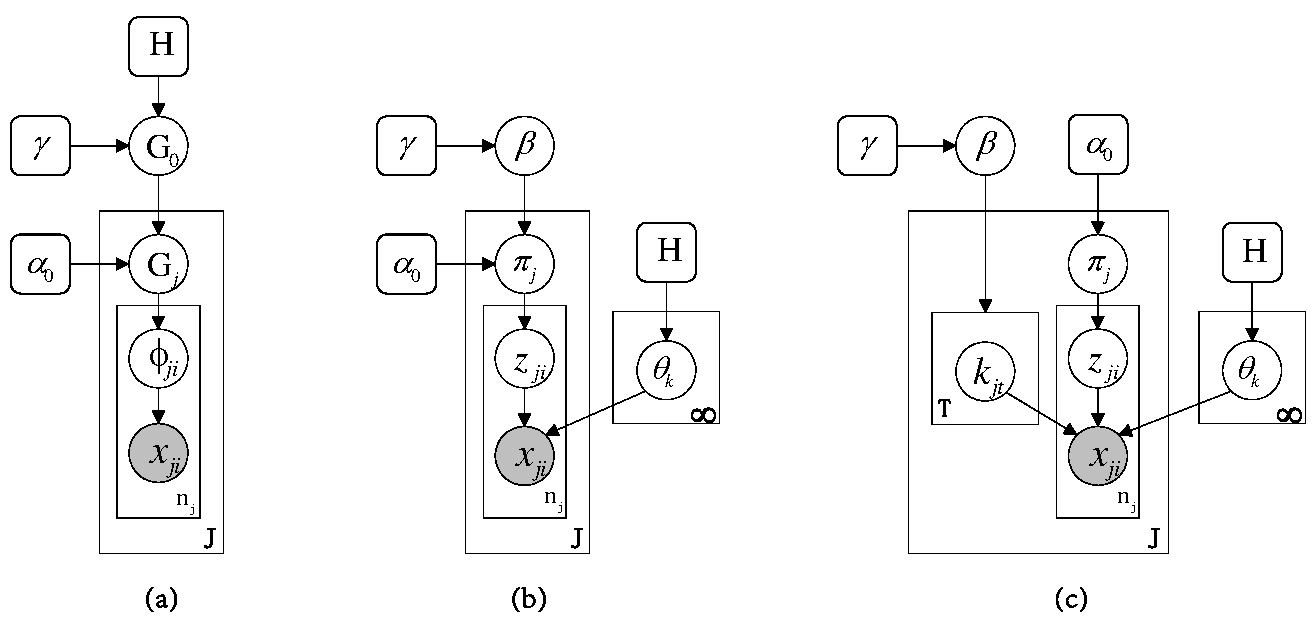
\includegraphics[angle=270,width=\textwidth]{hdp.pdf} 
\caption{HDP的图模型表示} \label{fig:hdp}
\end{figure}

这一模型称为分层Dirichlet过程模型(Hierarchical Dirichlet processes model,HDP)\cite{TEH:06},图\ref{fig:hdp}(a)给出了它的图模型表示。

\subsection{Stick-Breaking构造}

因为$G_0$服从$DP(\gamma,H)$,根据stick-breaking构造,$G_0$可以写成:
\begin{equation}
G_0 = \sum_{k=1}^{\infty}\beta_k\delta_{\theta_k}
\end{equation}
其中$\theta_k \sim H$,${\bm \beta} = {(\beta_i)}_{i=1}^\infty \sim Gem(\gamma)$。

可知$G_0$在${\bm \theta} = {(\theta_i)}_{i=1}^\infty$处有值,而每个$G_j$是服从$DP(\alpha_0,G_0)$的,所以每个$G_j$也在这些点处有值,$G_j$可写为:
\begin{equation}
G_j = \sum_{k=1}^{\infty}\pi_{jk}\delta_{\theta_k}
\end{equation}

记${\bm \pi}_j = {(\pi_{jk})}_{k=1}^\infty$。因为当给定$G_0$时$G_j$是相互独立的,所以当给定${\bm \beta}$时${\bm \pi}_j$是相互独立的。下面分析${\bm \pi}_j$和${\bm \beta}$的关系。
根据Dirichlet过程的定义,对于$\Theta$上的任意可测划分$(A_1,...,A_r)$,有:
\begin{equation}
(G_j(A_1),...,G_j(A_r)) \sim Dir(\alpha_0G_0(A_1),..., \alpha_0G_0(A_r))
\end{equation}
令$K_l = \{k:\theta_k \in A_l\},l = 1,...,r$,则有:
\begin{equation}
(\sum_{k \in K_1}\pi_{jk},...,\sum_{k \in K_r}\pi_{jk}) \sim Dir(\alpha_0\sum_{k \in K_1}\beta_{k},..., \alpha_0\sum_{k \in K_r}\beta_{k})
\end{equation}

成分变量$\phi_{ji}$是服从$G_j$分布的,且以概率$\pi_{jk}$的概率取到$\theta_k$,和Dirichlet过程(式\eqref{eq:dp_mix_sb})一样,用$z_{ji} =k $来指示$\phi_{ji} = \theta_k$,则HDP模型可以等价表示为:
\begin{equation}
\begin{split}
& {\bm \beta} \sim Gem(\gamma)\\
& {\bm \pi}_j \sim DP(\alpha_0,{\bm \beta})\\
& \theta_k \sim H\\
& z_{ji} \sim {\bm \pi}_j\\
& x_{ji} \sim F(\theta_{z_{ji}}) 
\end{split}
\label{eq:hdp_mix_sb}
\end{equation}
这一等价表示如图\ref{fig:hdp}(b)所示。

\subsection{连锁中国餐馆过程}
\begin{figure}
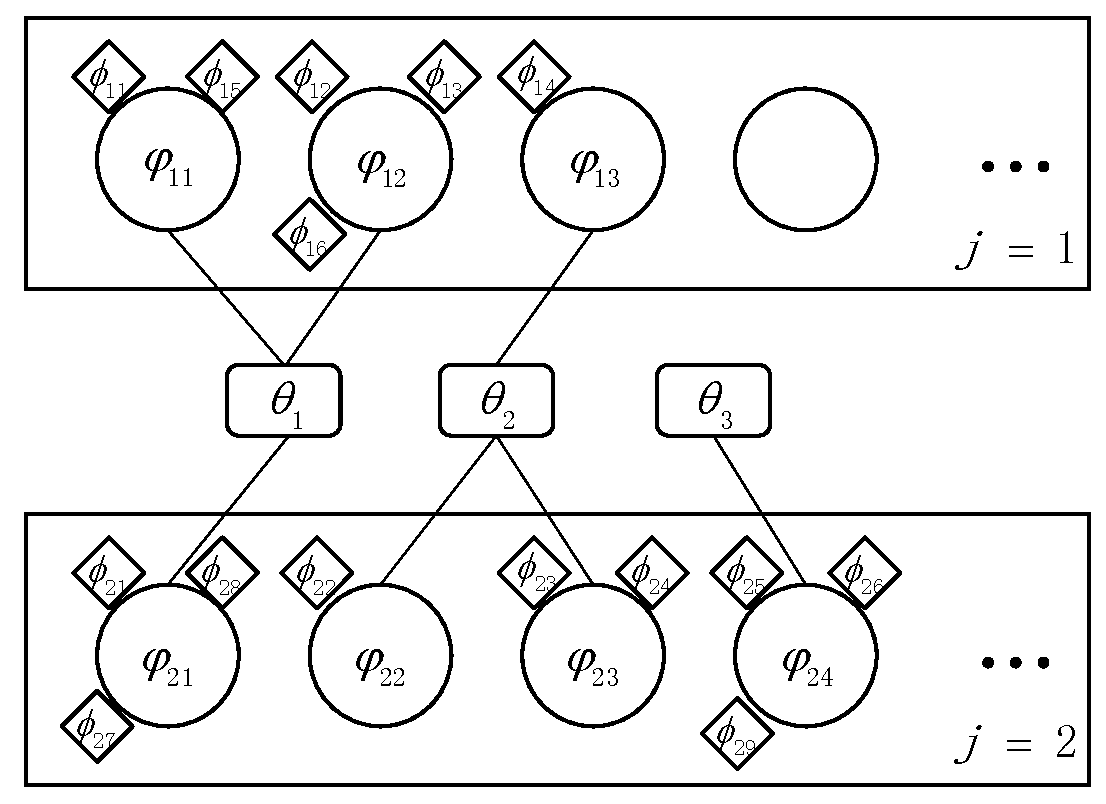
\includegraphics[angle=270,width=\textwidth]{CRF.pdf} 

  \caption{连锁中国餐馆过程示意图} \label{fig:CRF}
\end{figure}
在讨论Dirichlet过程时,用中国餐馆过程来描述其采样的预测分布,而此处的HDP模型中含有两层Dirichlet过程,也可以用类似的过程来描述。其对应的图模型如图\ref{fig:hdp}(c)所示。

沿用\ref{sec:dpm}节的定义,$\phi_{ji}$为第j组数据中$x_{ji}$对应的成分变量。这里令$\theta_1,...,\theta_K$表示全局已经出现过的成分变量,他们是独立同分布于H的,$\psi_{j1},...,\psi_{jT_j}$表示第j组数据中$T_j$个已经出现过的成分变量,他们是独立同分布于$G_0$的。

每个$\phi_{ji}$是和一个$\psi_{jt}$关联的,而每个$\psi_{jt}$是和一个$\theta_k$关联的。令$n_{jt}$表示和$\psi_{jt}$关联的$\phi_{ji}$的个数,$m_{jk}$表示第j组数据中和$\theta_k$关联的$\psi_{jt}$的个数,$m_k = \sum_{j}m_{jk}$表示和$\theta_k$关联的所有$\psi_{jt}$的个数。因为$G_j$和$G_0$都是服从Dirichlet过程的分布,$\phi_{ji}$和$\psi_{jt}$分别服从$G_j$和$G_0$,所以根据式\eqref{eq:crp_phi}可知:
\begin{equation}
p(\phi_{ji}|\phi_{j1},...,\phi_{j {i-1}},\alpha_0,G_0) = \frac{1}{\alpha_0+i-1}(\sum_{t=1}^{T_j}n_{jt}\delta_{\psi_{jt}} +\alpha_0G_0 ) \label{eq:crf_phi}
\end{equation}
\begin{equation}
p(\psi_{jt}|\psi_{11},\psi_{12},...,\psi_{21},...,\psi_{j {t-1}},\gamma,H) = \frac{1}{\sum_k{m_k}+\gamma}(\sum_{k=1}^{K}m_{k}\delta_{\theta_{k}} +\gamma H ) \label{eq:crf_psi}
\end{equation}

如果仿照式\eqref{eq:crp_z},用指示变量$t_{ji} = t$ 表示$\phi_{ji} = \psi_{jt}$,$k_{jt} = k$表示$\psi_{jt} = \theta_k$,则得到:
\begin{equation}
p(t_{ji}|t_{j1},...,t_{j {i-1}},\alpha_0) \propto \sum_{t=1}^{T_j}n_{jt}\delta_{t} +\alpha_0\delta_{t^{new}}\label{eq:crf_t}
\end{equation}
\begin{equation}
p(k_{jt}|k_{11},k_{12},...,k_{21},...,k{j {t-1}},\gamma) \propto \sum_{k=1}^{K}m_{k}\delta_{k} +\gamma\delta_{k^{new}}  \label{eq:crf_k}
\end{equation}

上面的过程称为连锁中国餐馆过程(Chinese restuarant franchise,CRF)。在这个比喻里面,假设一个中国餐馆连锁店有J家分店(每家分店对应一组数据),这些分店的菜单都是相同的且有无限种菜品(组间共享无限个成分),每个餐馆里每张桌子上只有一道菜,由第一个坐到这张桌子上的顾客点选,之后坐到这张桌子的所有顾客分享这一道菜。不同餐馆的桌子上可能会上同一道菜,而同一个餐馆上的不同桌子上也可能有同一道菜。模型里的$\phi_{ji}$对应着顾客,$\psi_{jt}$对应着桌子,$\theta_k$对应着菜。

当一位顾客进入第$j$家餐馆,他以某种概率坐在某张已经有人的桌子上,以剩余的概率坐在一张新的桌子上,这对应着式\eqref{eq:crf_phi},当他坐在一个新桌子上时,他会根据菜单中的菜在所有连锁店中的流行程度点一份新的菜,这对应着式\eqref{eq:crf_psi}。其示意图如图\ref{fig:CRF}所示。

\section{HDP的推断}
HDP的推断需要利用估计推断方法,本文主要介绍基于Gibbs sampling的方法\cite{NEAL:00,TEH:06}。
\subsection{基于CRF的采样方法}
在利用CRF描述的模型里,未知的随机变量是$\theta_k$,$\psi_{jt}$和$\phi_{ji}$。这里利用Gibbs采样的方法,根据每个变量在其他变量上的条件概率每次采样单个变量。由于$\theta_k$,$\psi_{jt}$和$\phi_{ji}$都是分布的参数,如高斯分布的均值和方差,如果直接采样,会需要大量的存储空间。所以,可以只采样$\theta_k$,而对于$\psi_{jt}$和$\phi_{ji}$,则通过采样相应的指示变量$k_{jt}$和$t_{ji}$得到,由于$\theta_k$的个数只有K个,采样过程更加有效。

这样,用于采样的状态空间变为了${\bm t}$,${\bm k}$,${\bm \theta}$,其中${\bm t}$的维数是固定的,即观察数,而${\bm k}$和${\bm \theta}$的维数是不固定的,所以采样空间是一个无限可数维度的。不过要注意,对于每一步采样而言,其维度是有限的。
\subparagraph{采样 t}
这里需要从$t_{ji}$在其他变量下的条件概率中采样$t_{ji}$。根据条件概率公式,只需计算$t_{ji}$的条件先验分布和生成$x_{ji}$的似然,即可得到$t_{ji}$的条件后验分布。
\begin{equation}
p(t_{ji}=t|{\bm t}^{-ji},{\bm k},{\bm \theta},{\bm x}) \propto p(t_{ji}=t|{\bm t}^{-ji})p(x_{ji}|t_{ji},{\bm k},{\bm \theta})
\end{equation}
式中右手第一项即条件先验概率,根据中国餐馆过程可知,$t_{ji}$等于一个已经存在的$t$的概率是正比于$n_{jt}^{-i}$的,而等于一个新的$t^{new}$的概率是正比于$\alpha_0$的。当$t_{ji}$等于一个已经存在的$t$时,$x_{ji}$的似然为$f(x_{ji}|\theta_{k_{jt}})$。当$t_{ji}$等于$t^{new}$时,情况要稍微复杂一些,这时需要为餐馆j采样出一个新的菜的$\psi_{jt^{new}}$,即采样出一个$k_{jt^{new}}$,如果$k_{jt^{new}}$是一个新的$k$,即$k_{jt^{new}} = K + 1$,则还要从基分布中生成一个新的$\theta$,其过程如下
\begin{equation}
k_{jt^{new}}|{\bm k} \sim \sum_{k=1}^{K}{ \frac{m_k}{\sum_{k}m_k + \gamma}\delta_k } +\frac{\gamma}{ \sum_{k}m_k + \gamma}\delta_{k^{new}}  , \theta_{k^{new}} \sim H \label{eq:hdp_sample_t_k} 
\end{equation}

此时$x_{ji}$的似然为$f(x_{ji}|\theta_{k_{jt^{new}}})$。故:
\begin{equation}\vspace{-5pt}
p(t_{ji} = t|{\bm t}^{-ji},{\bm k},{\bm \theta},{\bm x})\propto\left\{
\begin{array}{ll}
\alpha_0f(x_{ji}|\theta_{k_{jt}})  & t = t^{new},\\
n_{jt}^{-i}f(x_{ji}|\theta_{k_{jt}})  & \text{$t$为已经有顾客的餐桌}. 
\end{array}
\right.
\end{equation}

此处可以对$k_{jt^{new}}$进行平滑,即不是采样出一个新的k值,而是考虑在$k_{jt^{new}}$所有可能取值下的期望。此时似然函数为:
\begin{equation}
{\bm E}_{k_{jt^{new}}|{\bm k}}[f(x_{ji}|\theta_{k_{jt^{new}}})] = \sum_{k=1}^{K} {\frac{m_k}{\sum_{k} m_k + \gamma}f(x_{ji}|\theta_k) } +\frac{\gamma}{ \sum_{k}m_k + \gamma}f(x_{ji}|\theta_{k^{new}}). \label{eq:hdp_smoothing_k} 
\end{equation}
\subparagraph{采样 $k$}
采样$k_{jt}$和采样$t_{ji}$的过程类似,区别在于似然函数上,对于$t_{ji}$采样时,和$t_{ji}$相关的$x$只有$x_{ji}$,而对于$k_{jt}$,他的采样值会影响到第$j$个餐馆第$t$个桌上所有的$x_{ji}$(即$t_{ji} = t$的$x_{ji}$),所以其似然部分为$\prod_{i:t_{ji}=t}f(x_{ji}|\theta_k)$.故:
\begin{equation}\vspace{-5pt}
p(k_{jt} = k|{\bm t},{\bm k}^{-jt},{\bm \theta},{\bm x})\propto\left\{
\begin{array}{ll}
\gamma\prod_{i:t_{ji}=t}f(x_{ji}|\theta_k)  & k = k^{new},\\
m_{k}^{-t}\prod_{i:t_{ji}=t}f(x_{ji}|\theta_k)  & \text{$k$为已经有顾客点过的菜}.
\end{array}
\right.
\end{equation}
\subparagraph{采样 $\theta$}
$\theta_k$的取值会影响到所有和$\phi_{ji} = \theta_k$(即$k_{jt_{ji}}=k$)的$x_{ji}$的似然,所以$\theta_k$的后验分布如下:
\begin{equation}
p(\theta_k|{\bm t},{\bm k},{\bm \theta^{-k}},{\bm x}) \propto h(\theta_k) \prod_{ji:k_{jt_{ji}}=k}f(x_{ji}|\theta_k)
\end{equation}
\subparagraph{collapsed gibbs采样}
如果$H$是$f(\theta)$的共轭先验,比如$H$是Dirichlet分布而$f(\theta)$是多项分布,则可以利用边缘概率公式$\theta$消去,利用collapsed Gibbs采样加快采样的收敛速度。

首先考虑采样$t_{ji}$时需要计算的似然。当$\theta_k$已知时,$x_{ji}$的似然为$f(x_{ji}|\theta_k)$,而当不对$\theta_k$进行采样时,根据式\eqref{eq:finite_collapsed_gibbs_pi_theta},则需要计算$x_{ji}$在${\bm x}^{-ji}$上的后验分布:
\begin{equation}
f_k(x_{ji}|{\bm x}^{-ji}) = \frac{\int f(x_{ji}|\theta_k)\prod_{{j^\prime}{i^\prime}\neq ji,z_{{j^\prime}{i^\prime}}=k} f(x_{{j^\prime}{i^\prime}}|\theta_k)H(\theta_k) d\theta_k}{\int \prod_{{j^\prime}{i^\prime}\neq ji,z_{{j^\prime}{i^\prime}}=k} f(x_{{j^\prime}{i^\prime}}|\theta_k) H(\theta_k) d\theta_k } \label{eq:collapsed_k_single} 
\end{equation}
其中$z_{ji} = k_{jt_{ji}}$。
\label{eq:hdp_sample_t_k} 
若$k=k^{new}$,此时的后验分布为$\int f(x_{ji}|\theta_k)H(\theta_k) d\theta_k$。

当$t_{ji}$的采样为$t^{new}$时,可以根据式\eqref{eq:hdp_sample_t_k}采样出一个$k_{jt^{new}}$,如果$k_{jt^{new}}$是一个新的$k^{new}$,则此时的似然为$\int f(x_{ji}|\theta_k)H(\theta_k) d\theta_k$。

如果使用式\eqref{eq:hdp_smoothing_k}中的平滑算法,则此时该式变为:
\begin{equation}
{\bm E}_{k_{jt^{new}}|{\bm k}}[f(x_{ji}|{\bm x}^{-ji})] = \sum_{k=1}^{K} {\frac{m_k}{\sum_{k} m_k + \gamma}f_k(x_{ji}|{\bm x}^{-ji}) } +\frac{\gamma}{ \sum_{k}m_k + \gamma}f_{k^{new}}(x_{ji}|{\bm x}^{-ji})
\end{equation}

在采样$k_{jt}$时,需要计算第$j$个餐馆第$t$个桌子上所有$x$的似然,记作${\bm x}_{jt}$,这时后验分布变成了:
\begin{equation} hbf01214_k({\bm x}_{jt}|{\bm x}^{-jt}) = \frac{\int f({\bm x}_{jt}|\theta_k)\prod_{{j^\prime}{i^\prime}\neq ji,z_{{j^\prime}{i^\prime}}=k}f(x_{{j^\prime}{i^\prime}}|\theta_k)H(\theta_k) d\theta_k}{\int \prod_{{j^\prime}{i^\prime}\neq ji,z_{{j^\prime}{i^\prime}}=k}f(x_{{j^\prime}{i^\prime}}|\theta_k)H(\theta_k) d\theta_k}  \label{eq:collapsed_k_mult}
\end{equation}

若$k_{jt}=k^{new}$,此时的后验分布为$\int \prod_{t_{ji}=t}{f(x_{ji}}|\theta_k)H(\theta_k) d\theta_k$。

若H是参数为$\eta$的Dirichlet分布而$f(\theta)$是多项分布,则式\eqref{eq:collapsed_k_mult}变为:
\begin{equation}
f_k({\bm x}_{jt}|{\bm x}^{-jt}) = \frac{\Gamma(n_{k}^{-{\bm x}_{jt}} + V\eta)} {\Gamma(n_{k}^{-{\bm x}_{jt}} + n^{{\bm x}_{jt}} + V\eta)} \frac{\prod_v\Gamma(n_{kv}^{-{\bm x}_{jt}} + n_v^{{\bm x}_{jt}} + \eta)} {\prod_v\Gamma(n_{kv}^{-{\bm x}_{jt}}  + \eta)} \label{eq:collapsed_k_mult_r} 
\end{equation}

其中$n_{kv}^{-{\bm x}_{jt}}$表示除了${\bm x}_{jt}$以外,满足$x_{ji}=v,k_{ji} = k$的$x_{ji}$的个数。$n_{k}^{-{\bm x}_{jt}}$表示除了${\bm x}_{jt}$以外,满足$k_{ji} = k$的$x_{ji}$的个数。$n_{v}^{{\bm x}_{jt}}$表示满足$t_{ji}=t, x_{ji}=v$的$x_{ji}$的个数。$n^{{\bm x}_{jt}}$表示满足$t_{ji}=t$的$x_{ji}$的个数。V表示多项分布的维数。

而式\eqref{eq:collapsed_k_single}只是式\eqref{eq:collapsed_k_mult}的一个特殊情况:
\begin{equation}
f_k(x_{ji}=v|{\bm x}^{-ji}) = \frac{n_{kv}^{-x_{ji}} + \eta}{n_{kv}^{-x_{ji}} + V\eta}\label{eq:collapsed_k_single_r} 
\end{equation}

\subsection{直接分配采样方法}\label{subsec:direct_assignment_sample}
除了从基于中国餐馆过程的表示得到采样算法,也可以从基于stick-breaking的表示(式\eqref{eq:dp_mix_sb})得到HDP的另一种采样方法。这里直接用$z_{ji}$来表示$x_{ji}$和$\theta_k$的对应关系,故本文称其为直接分配采样方法\cite{TEH:06,heinrich:2011,zhou2011}。

根据模型,需要采样的变量有${\bm z}$,${\bm \pi}$,${\bm \beta}$和${\bm \theta}$。由于${\bm \pi_j}$服从Dirichlet分布,而其是多项分布($z_{ji}$服从一个参数为${\bm \pi_j}$的多项分布)的共轭先验,类似于式\eqref{eq:finite_collapsed_gibbs_pi},将${\bm \pi}$积分掉,只对${\bm z}$,${\bm \beta}$以及${\bm \theta}$进行Gibbs采样。为了使得采样过程可行,只考虑当前模型中已有的K个混合成分(有限个),而对于其他所有仍未出现的成分(无限个),并不显式表示出每一个成分,而是用单个变量来记录。这里将模型中已有的K个混合成分对应的${\bm \beta}$记为$\beta_1$到$\beta_K$,而将其他所有没有出现的成分记为$\beta_u = \sum_{k=K+1}^{L}\beta_k$。这样采样过程中的${\bm \beta}$为$(\beta_1,...,\beta_K,...\beta_u)$。当采样到一个新的混合成分时,对K增加1,而对用来记录未出现成分的变量进行更新。

\subparagraph{采样${\bm z}$}
根据Dirichlet分布和多项分布的共轭性质,参考式\eqref{eq:collapsed_k_single_r},得到${z_{ji}}$在${\bm z}^{-ji}$和${\bm \beta}$条件下的先验分布:
\begin{equation}
f_k(z_{ji}=k|{\bm z}^{-ji},{\bm \beta}) = \frac{n_{jk}^{-z_{ji}} + \alpha_0\beta_k}{n_j^{-z_{ji}} + K\alpha_0\beta_k} \label{eq:piror_z} 
\end{equation}
该式分母对于不同的k值是个常量,故可以省去,根据$x_{ji}$的条件分布,得到$z_{ji}$的后验概率为:
\begin{equation}
f_k(z_{ji}=k|{\bm z}^{-ji},{\bm \beta},{\bm \theta},{\bm x}) \propto (n_{jk}^{-z_{ji}} + \alpha_0\beta_k)f(x_{ji}|\theta_k)\label{eq:sample_z} 
\end{equation}

\subparagraph{采样${\bm \beta}$}
利用Dirichlet分布和多项分布的共轭性质,得到:
\begin{equation}
p({\bm z}|{\bm \beta}) = \prod_{j=1}^{J}\frac{\Gamma(\alpha_0)}{\Gamma(\alpha_0 + n_j)} \prod_{k=1}^{K}\frac{\Gamma(\alpha_0\beta_k+n_{jk})}{\Gamma(\alpha_0\beta_k)} \label{eq:z_cond_beta}
\end{equation}
这个式子可以看做是${\bm \beta}$的似然函数,注意其中${\bm \beta}$出现在$\Gamma$函数中,所以联合${\bm \beta}$的先验得到的$p({\bm \beta}|{\bm z})$并不是一个指数函数族分布,难以从中直接采样出${\bm \beta}$。所以下面通过引入一个辅助变量,构造出一个满足指数族分布的后验概率来采样${\bm \beta}$。

对于式\eqref{eq:z_cond_beta}中的第二项,可以展开为关于$\alpha_0\beta_k$的多项式函数:
\begin{equation}
\frac{\Gamma(\alpha_0\beta_k+n_{jk})}{\Gamma(\alpha_0\beta_k)} = \prod_{m_{jk}=1}^{n_{jk}}(m_{jk}-1+\alpha_0\beta_k) = \sum_{m_{jk}=0}^{n_{jk}} s(n_{jk},m_{jk}){(\alpha_0\beta_k)}^m_{jk}
\end{equation}
其中$s(n_{jk},m_{jk})$为第一类Stirling数,${\bm m} = (m_{jk})$是引入的一个辅助变量。

这里构造一个关于${\bm z}$,${\bm m}$和${\bm \beta}$的分布:
\begin{equation}
q({\bm z,m,\beta}) = \frac{\Gamma(\gamma)}{\Gamma(\gamma_r)\Gamma(r_u)}(\sum_{j=1}^J\frac{\Gamma(\alpha_0)}{\Gamma(\alpha_0+n_j)})\beta_u^{\gamma_u-1}\prod_{k=1}^{K}\beta_k^{\gamma_r-1}\prod_{j=1}^{J}(\alpha_0\beta_k)^{m_{jk}}s(n_{jk},m_{jk})
\end{equation}

可以验证,$\sum_m q({\bm z},{\bm m},{\bm \beta}) = p({\bm z},{\bm \beta})$,所以从分布q采样得到的${\bm \beta}$是和从分布$p({\bm \beta},{\bm z})$中采样的${\bm \beta}$一致的,从而可以利用这一构造建立一个基于辅助变量${\bm m}$的采样方法来采样${\bm \beta}$:
\begin{equation}
q(m_{jk} = m|{\bm z,m_{-jk},\beta}|) \propto s(n_{jk},m)(\alpha_0\beta_k)^m \label{eq:m_cond_beta}
\end{equation}
\begin{equation} 
q({\bm \beta}|{\bm z,m}) \propto \beta_u^{\gamma-1}\prod_{k=1}^{K}\beta_k^{{\sum_{j}m_{jk}}-1} \label{eq:beta_cond_m}
\end{equation} 

回忆CRF构造中已经使用了$m_{jk}$来表示第$j$个餐馆中上了第$k$道菜的桌子的个数。这里的辅助变量也使用的相同的记号,其实两个记号一致并不是巧合,他们正是同一个变量,但是由于在直接分配的方法中,是直接采样的$z_{ji}$,因为有可能同一餐馆的两个不同桌子都是点的第$k$道菜,所以无法计算出$m_{jk}$,而只能去计算它的概率。下面给出证明。

考虑第j个餐馆的采样过程,并且只考虑顾客被安排到点了第k道菜的桌子(即所有$k_{jt}=k$的桌子t)的情况,这可以看做是第j个餐馆的完整采样过程的一个子情况,其先验概率如下:
\begin{equation}\vspace{-5pt}
p(t_{ji} = t|{\bm t}^{-ji},k_{jt}=k,{\bm \beta},{\bm x})\propto\left\{
\begin{array}{ll}
\alpha_0\beta_k  & t = t^{new},\\
n_{jt}^{-i}  & \text{$t$为已经有顾客的餐桌}. 
\end{array}
\right.
\end{equation}
可以看出,这个子情况可以等价为一个中心参数为$\alpha_0\beta_k$的Dirichlet过程对应的中国餐馆过程。根据Antoniak定理(式\eqref{eq:antoniak}),对于一个Dirichlet过程,如果知道当前的总采样数,则可以得到一个关于其当前的成分个数的分布。上述过程的总采样数为$n_{jk} = \sum_{k_{jt}=k}{n_{jt}}$,其成分个数则是餐馆j中所有$k_{jt}=k$的桌子个数,即$m_{jk}$,从而有:
\begin{equation}
p(m_{jk} = m|\text{采样数为}n_{jk},\alpha_0\beta_k) = s(n_{jk},m)(\alpha_0\beta_k)^m\frac{\Gamma(\alpha_0\beta_k)}{\Gamma(\alpha_0\beta_k+n_{jk})}  \label{eq:component_num_dis}
\end{equation}
此式和式\eqref{eq:m_cond_beta}一致,说明辅助变量$m_{jk}$和中国CRF中的$m_{jk}$是一致的。

这也说明,当采用基于CRF的采样方法时,如果需要采样${\bm \beta}$,可以直接使用$m_{jk}$。

这里再介绍另一种推导${\bm \beta}$采样公式的方法。假设当前已经有的K个不同的菜品将${\bm \Theta}$划分为${\{\theta_1,\theta_2,\...\theta_K,\theta_{\tilde{k}}\}}$,其中${\theta_{\tilde{k}} = {\bm \Theta} \backslash \bigcup_{k=1}^K\{\theta_k\}}$是当前还没出现过的参数。根据DP的定义,有
\begin{equation}
\begin{aligned}
(G_0(\theta_1),...,G_0(\theta_K),G_0({\theta_{\tilde{k}}})) &\sim Dir(\gamma H(\theta_1),..., \gamma H(\theta_K),\gamma H ({\theta_{\tilde{k}}}) ) \\
													& \sim Dir(0,...,0,\gamma)
\end{aligned}
\end{equation}
注意,其中H是连续空间上的测度,所以在参数点上的测度为0。假设第j个餐馆第t个桌子上的菜是$\psi_{jt}$,则有
\begin{equation}
p(G_0(\theta_1),...,G_0(\theta_K),G_0({\theta_{\tilde{k}}})|\{\psi_{jt}\}),\gamma) \propto Dir(\sum_{j}m_{j1}...\sum_{j}m_{jK},\gamma) 
\end{equation}
根据定义,可知$(G_0(\theta_1),...,G_0(\theta_K),G_0({\theta_{\tilde{k}}}))$就是${\bm \beta}$。这样得到和式\eqref{eq:beta_cond_m}一致的采样公式。

\subparagraph{采样${\bm \theta}$}
对于${\bm \theta}$的采样和基于CRF的采样方法中的一致:
\begin{equation}
p(\theta_k|{\bm t},{\bm k},{\bm \theta^{-k}},{\bm x}) \propto h(\theta_k) \prod_{ji:z_{ji}=k}f(x_{ji}|\theta_k)
\end{equation}
同样,和基于CRF的采样方法一样,如果$H$是$f(\theta)$的共轭先验,也可以进一步将${\bm \theta}$积分掉,进而只对${\bm z}$,${\bm \beta}$进行Gibbs采样。

\subparagraph{采样${\bm \pi}$}
前面在采样${\bm z}$和${\bm \beta}$时将${\bm \pi}$积分掉来加快采样速度,但是有些时候需要采样${\bm \pi}$的值,比如在对多文档建模时${\bm \pi}$可以用来表征文档在主题层的表示\cite{blei2003latent}。根据共轭性质,其后验分布如下:
\begin{equation}
p({\bm \pi}|{\bm z,\beta}) \propto \prod_{j=1}^{J}{{\pi_{ju}}^{\alpha_0\beta_u-1}  \prod_{k=1}^{K}{\pi_{jk}^{\alpha_0\beta_k+n_{jk}-1}} }
\end{equation}

\subsection{超参数的更新}\label{subsec:hdp_hyper}
模型含有两个超参数$\gamma$和$\alpha_0$,无论是用哪种采样方法,都需要对其进行更新。这里为这两个参数加上先验,然后根据参数的后验概率进行采样。
\subparagraph{$\alpha_0$的采样}
根据式\eqref{eq:component_num_dis},可以得到:
\begin{equation}
p(T_1,...,T_J|\alpha_0,n_1,...,n_J) = \prod_{j=1}^J{s(n_{j},T_j)(\alpha_0)^{T_j}\frac{\Gamma(\alpha_0)}{\Gamma(\alpha_0+n_j)}} \label{T_antoniak}
\end{equation} 

这里$T_j$是第$j$个餐馆的桌子个数,$n_j$是第$j$个餐馆当前观察的总数。当观察到$T_j$时,$X$是独立于$\alpha_0$的,所以上式可以看做求$\alpha_0$后验时需要的似然函数,在联合$\alpha_0$的先验,就可以得到$\alpha_0$的后验概率,从而可以进行采样更新。

假设$\alpha_0$的先验是一个参数为$a$和$b$的$gamma$分布,则${\alpha_0}$的后验为:
\begin{equation}
p(\alpha_0|T_1,...,T_j,a,b) \propto  {\alpha_0}^{a-1+\sum_{j=1}^J{T_j}} e^{\alpha_0b} \prod_{j=1}^J{s(n_{j},T_j)\frac{\Gamma(\alpha_0)}{\Gamma(\alpha_0+n_j)}}
\end{equation} 

由于$\alpha_0$出现在$\frac{\Gamma(\alpha_0)}{\Gamma(\alpha_0+n_j)}$中,导致这个后验概率不服从指数族分布。这里使用West等人提出的一种基于辅助变量的方法\cite{west:92,escobar:95,rasmussen:99},使得$\alpha_0$在辅助变量下的后验是服从指数族分布的,从而可以进行采样更新。

首先考虑$\frac{\Gamma(\alpha_0)}{\Gamma(\alpha_0+n_j)}$,可以将其展开成:
\begin{equation}
\frac{\Gamma(\alpha_0)}{\Gamma(\alpha_0+n_j)} = \int_0^1{{w_j}^{\alpha_0}(1-w_j)^{n_j-1}(1+\frac{n_j}{\alpha_0})} d{w_j}
\end{equation} 

这里定义辅助变量${\bm w} = (w_j)_{j=1}^J$和${\bm s} = (s_j)_{j=1}^J$,其中$w_j$在$[0,1]$之间取值而$s_j$是一个只能取${0,1}$的二值变量。定义分布:
\begin{equation}
q(\alpha_0,{\bm w,s}) \propto {\alpha_0}^{a-1+\sum_{j=1}^J{T_j}} e^{\alpha_0b} \prod_{j=1}^J{{w_j}^{\alpha_0}(1-w_j)^{n_j-1}{(\frac{n_j}{\alpha_0})}^{s_j}}
\end{equation} 

可以验证,积分掉${\bm w}$和${\bm s}$,得到的正是$\alpha_0$的后验分布:
\begin{equation}
\int q(\alpha_0,{\bm w,s}) d{\bm w}d{\bm s} = p(\alpha_0|T_1,...,T_j,a,b) 
\end{equation} 

从而,可以对三个变量分别进行采样,得到$\alpha_0$的采样方法:
\begin{equation}
\begin{split}
& q(\alpha_0|{\bm w,s}) \propto {\alpha_0}^{a-1+\sum_{j=1}^J{T_j-s_j}} e^{\alpha_0(b-\sum_{j=1}^J \ln{w_j})}\\
& q(w_j|\alpha_0) \propto {w_j}^{\alpha_0}{(1-w_j)}^{n_j-1} \quad j \in \{1,...,J\}\\
& q(s_j|\alpha_0) \propto (\frac{n_j}{\alpha_0})^{s_j} \quad j \in \{1,...,J\}
\end{split}
\end{equation} 

从三个变量的后验概率形式可以看出,$\alpha_0$服从$gamma$分布,$w_j$服从dirichlet分布,$s_j$服从bernoulli分布。

\subparagraph{$\gamma$的采样}
对于参数$\gamma$,可以得到:
\begin{equation}
p(K|\gamma,T) = s(T,K) \gamma_K \frac{\Gamma(\gamma)}{\Gamma(\gamma + T) }
\end{equation} 
其中$T = \sum_j{T_j}$是总桌子数,而$K$是模型中的不同成分个数,即不同种类菜的个数。这个式子和式\eqref{T_antoniak}一致,从而可以使用与上面更新$\alpha_0$完全一样的方法来更新$\gamma$。

注意,一般先对变量采样多次,然后更新一遍参数。
